%
% domain.tex -- graph of characteristics in problem 90000020
%
% (c) 2019 Prof Dr Andreas Müller, Hochschule Rapperswil
%
\documentclass[tikz,12pt]{standalone}
\usepackage{amsmath}
\usepackage{times}
\usepackage{txfonts}
\usepackage{pgfplots}
\usepackage{csvsimple}
\usetikzlibrary{arrows,intersections,math}
\begin{document}
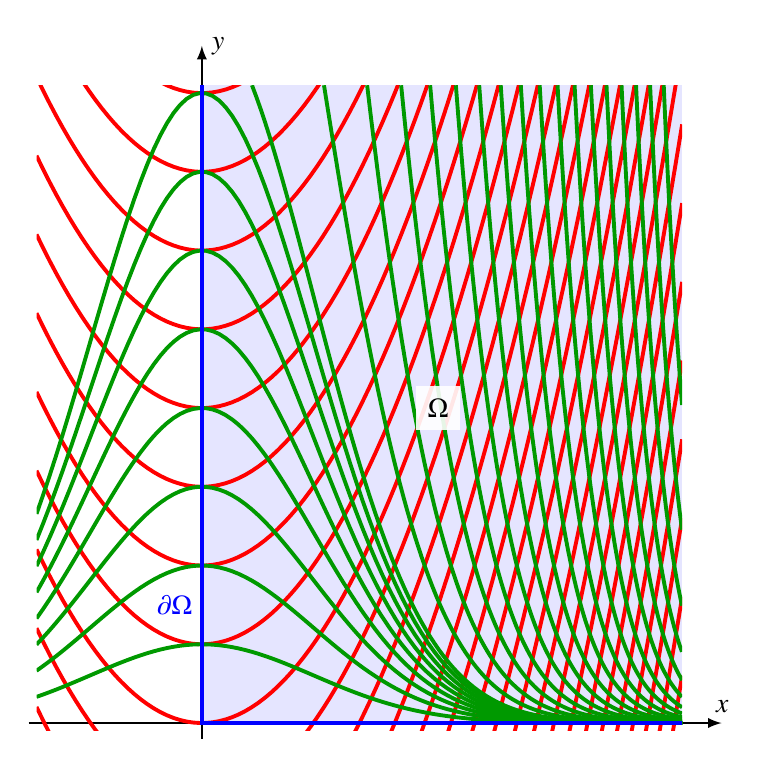
\begin{tikzpicture}[>=latex,scale=2]

\definecolor{darkgreen}{rgb}{0,0.6,0}

\fill[color=blue!10] (0,0) rectangle (3.05,4.05);

\draw[->,line width=0.7pt] (-1.1,0)--(3.3,0) coordinate[label={$x$}];
\draw[->,line width=0.7pt] (0,-0.1)--(0,4.3) coordinate[label={right:$y$}];

\begin{scope}
\clip (-1.05,-0.05) rectangle (3.05,4.05);
\foreach \C in {-9,-8.5,...,4}{
	\draw[color=red,line width=1.4pt]
		plot[domain=-1.05:3.05,samples=100] ({\x},{\x*\x+\C});
}
\foreach \D in {0.5,1,...,4}{
	\draw[color=darkgreen,line width=1.4pt]
		plot[domain=-1.05:3.05,samples=100] ({\x},{\D*exp(-\x*\x)});
}
\foreach \k in {1.5,2,...,10}{
	\draw[color=darkgreen,line width=1.4pt]
		plot[domain={sqrt(-ln(4.05)+\k)}:3.05,samples=100]
			({\x},{exp(\k-\x*\x)});
}
\end{scope}

\draw[color=blue,line width=1.4pt] (0,4.05)--(0,0)--(3.05,0);
\node[color=blue] at (0,0.75) [left] {$\partial\Omega$};

\def\w{0.14}
\def\h{0.14}
\fill[color=white,opacity=0.9] ({1.5-\w},{2-\h}) rectangle ({1.5+\w},{2+\h});
\node at (1.5,2.0) {$\Omega$};

\end{tikzpicture}
\end{document}

